\paragraph{Validation iteration profiles.}
For SDF / SIREN, the QuotientOpt validation tuning profile reaches $10^{-4}$ of the common initial validation MSE at epoch 1142, whereas AdamW does not reach this target within 2000 epochs.
For Matrix completion, the QuotientOpt validation tuning profile reaches $10^{-4}$ of the common initial validation MSE at epoch 107, compared with epoch 138 for AdamW.
This is a descriptive validation-selected iteration comparison over equal 13-setting budgets, including finite checkpoints from stopped trials. It is not a wall-clock or single-trajectory speed claim. All three controls, every regression task, and all five targets are retained in Table~\ref{tab:new-task-hitting} and Figure~\ref{fig:new-task-convergence}.
\begin{figure}[t]
\centering
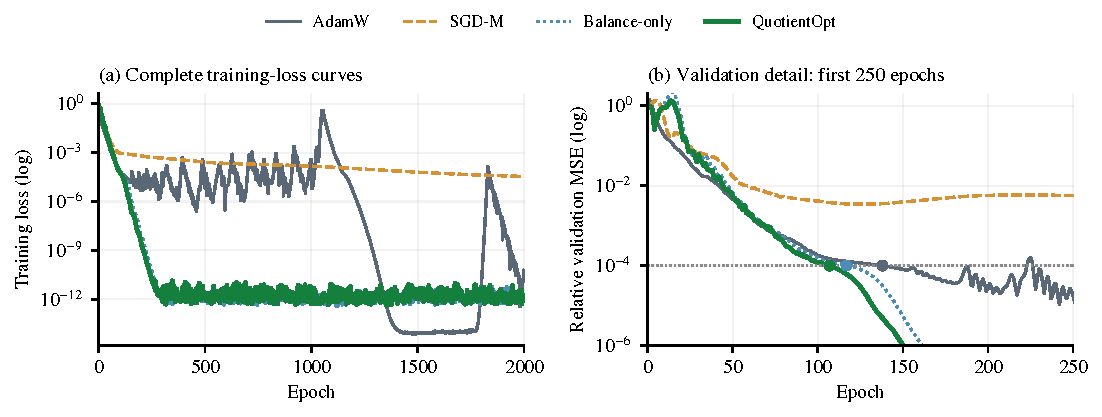
\includegraphics[width=.99\linewidth]{figures/new_matrix_convergence_raw.pdf}
\caption{\textbf{Additional matrix-completion loss curves.} Rank 8, planted condition 100, $128\times128$, seed 42. Each method selects its setting by the earliest validation epoch reaching $10^{-4}$ of the common initial validation MSE, over the same 13-setting budget. For SGD-M, which never reaches the target, the minimum-validation-loss full-horizon setting is shown. (a) Complete raw training-loss observations, without smoothing. (b) A common first-250-epoch validation zoom, with first-hitting points and the target line. These are actual selected-run trajectories. Figure~\ref{fig:new-task-convergence} separately reports tuning envelopes; the full record includes every setting and stopped prefix.}
\label{fig:new-matrix-raw}
\end{figure}
